%%% template.tex
%%%
%%% This LaTeX source document can be used as the basis for your technical
%%% paper or abstract.

%%% The parameter to the ``documentclass'' command is very important.
%%% - use ``e'' for content submitted for review.
%%% - use ``preprint'' for accepted content you are making available.
%%% - use ``tog'' for technical papers accepted to the TOG journal and
%%%   for presentation at the SIGGRAPH or SIGGRAPH Asia conference.
%%% - use ``conference'' for final content accepted to a sponsored event
%%%   (hint: If you don't know, you should use ``conference.'')

% \documentclass[tog]{acmsiggraph}

% \usepackage[numbered]{algorithm}
% \usepackage[noend]{algorithmic}
% \usepackage[super]{nth}

% %%% Make the ``BibTeX'' word pretty...

% \def\BibTeX{{\rm B\kern-.05em{\sc i\kern-.025em b}\kern-.08em
%     T\kern-.1667em\lower.7ex\hbox{E}\kern-.125emX}}

% %%% Used by the ``review'' variation; the online ID will be printed on 
% %%% every page of the content.

% \TOGonlineid{0214}

% %%% Used by the ``preprint'' variation.

% \TOGvolume{0}
% \TOGnumber{0}

% \title{An Interactive Tool for Designing Quadrotor Camera Shots\\Supplementary Material}

% \author{Niels Joubert\thanks{Niels Joubert and Mike Roberts contributed equally to this work.}\\Stanford University \and Mike Roberts$^{*}$\\Stanford University \and Anh Truong\\Stanford University \and Floraine Berthouzoz\\Adobe Research \and Pat Hanrahan\\Stanford University}
% \pdfauthor{Niels Joubert, Mike Roberts, Anh Truong, Floraine Berthouzoz, Pat Hanrahan}

% \floatstyle{boxed}
% \newfloat{Listing}{t}{ext}

% \renewcommand{\algorithmicrequire}{\small\textbf{Input:}}
% \renewcommand{\algorithmicensure}{\small\textbf{Output:}}

% \DeclareMathOperator*{\argmin}{arg\,min}
% \usepackage{amstext}

% \begin{document}

% \maketitle

%\begin{CRcatlist}
%  \CRcat{I.3.3}{Computer Graphics}{Three-Dimensional Graphics and Realism}{Display Algorithms}
%  \CRcat{I.3.7}{Computer Graphics}{Three-Dimensional Graphics and Realism}{Radiosity};
%\end{CRcatlist}

%\TOGlinkslist
%\copyrightspace

%\section{Specification Sheet for the \textsc{IRIS} Camera Control System by \textsc{Bot \& Dolly}}

%\begin{figure*}[t]
%  \centering
%  \includegraphics[width=7.0in]{images/iris}
%  \caption{
%Specification sheet for the \textsc{IRIS} camera control system developed by \textsc{Bot \& Dolly}. This brochure owned by Bot \& Dolly, reproduced here for education purposes to aid our related work discussion of systems comparable to ours.
%}
%  \label{figure:iris}
%\end{figure*}

%\textsc{Bot \& Dolly}, the company that developed the \textsc{IRIS} camera control system, is now defunct.
%The specification sheet for the \textsc{IRIS} camera control system is no longer available online.
%We include it in Figure \ref{figure:iris} in this document for completeness.

\subsection{Deriving the Quadrotor Camera Manipulator Matrices}
\label{sec:ch2:manipulator_detail}

In this subsection, we derive the manipulator matrices for our quadrotor camera model.
At a high level, our strategy will be to relate our quadrotor camera's degrees of freedom to our control inputs.

In the derivation that follows, we assume that our quadrotor and gimbal are \emph{kinematically coupled} \cite{kondak:2013}, in the sense that moving the position of the quadrotor also moves the position of the gimbal. However, we assume that our quadrotor and gimbal are not \emph{dynamically coupled} \cite{kondak:2013}, in the sense that torques acting on the gimbal do not induce reactive torques on the quadrotor.
These assumptions simplify the modeling of our system. Moreover, we feel they are justified, since in the cameras mounted on quadrotors tend to be very lightweight relative to the quadrotors themselves. For example, on our hardware platform, our camera and gimbal are roughly 25$\times$ lighter than our quadrotor.

\paragraph{Relating the Quadrotor's Position to the Control Inputs}

We assume that there are two forces acting on our quadrotor camera: (1) a \emph{thrust force} induced by the quadrotor's propellers; and (2) an \emph{external force} that models any other forces acting on the quadrotor, such as gravity, wind, and drag.
Based on this assumption, we use Newton's Second Law to relate the linear acceleration of the quadrotor in the world frame, $\ddot{\mathbf{p}}$, to the control input applied at each of the quadrotor's propellers, $\mathbf{u}_q$, as follows,
%
\begin{equation}
m \ddot{\mathbf{p}} = \mathbf{f}_e + \mathbf{R}_{\mathcal{W},\mathcal{Q}} \mathbf{M}_{\mathbf{f}} \mathbf{u}_q
\label{eqn:ch2:m_p_dot_dot}
\end{equation}
%
where $m$ is the mass of the quadrotor camera; $\mathbf{f}_e$ is the external force; $\mathbf{M}_{\mathbf{f}}$ is the matrix that maps the control input at each of the quadrotor's propellers into a net thrust force oriented along the quadrotor's local $\mathbf{y}$ axis; and $\mathbf{R}_{\mathcal{W},\mathcal{Q}}$ is the rotation matrix that represents the quadrotor's orientation in the world frame (i.e., the rotation matrix that maps vectors from the body frame of the quadrotor into the world frame).
We define $\mathbf{M}_{\mathbf{f}}$ as follows, 
%
\begin{equation}
\begin{aligned}
%
\mathbf{M}_{\mathbf{f}} =
\begin{bmatrix}
0 & 0 & 0 & 0 \\
1 & 1 & 1 & 1 \\
0 & 0 & 0 & 0 \\
\end{bmatrix}
%
\end{aligned}
\end{equation}

\paragraph{Relating the Quadrotor's Angular Acceleration and Angular Velocity to the Control Inputs}

We use Euler's Second Law to relate the angular acceleration and angular velocity of the quadrotor in the body frame, $\dot{\mathbf{\omega}}_q$ and $\mathbf{\omega}_q$ respectively, to the control input applied at each of the quadrotor's propellers, $\mathbf{u}_q$, as follows,
%
\begin{equation}
\mathbf{I}_{q} \dot{\mathbf{\omega}}_q + \mathbf{\omega}_q \times \mathbf{I}_q \mathbf{\omega}_q = \mathbf{M}_{\mathbf{\tau}} \mathbf{u}_q
\label{eqn:ch2:M_t_u_q_short}
\end{equation}
%
where $\mathbf{I}_{q}$ is the inertia matrix of the quadrotor camera; and $\mathbf{M}_{\mathbf{\tau}}$ is the matrix that maps the control input at each of the quadrotor's propellers into a net torque acting on the quadrotor in the body frame.
We define $\mathbf{M}_{\mathbf{\tau}}$ as follows, 
%
\begin{equation}
\begin{aligned}
%
\mathbf{M}_{\mathbf{\tau}} =
\begin{bmatrix}
 ds_\alpha & ds_\beta & -ds_\beta & -ds_\alpha \\
\gamma     & -\gamma  & \gamma    & -\gamma    \\
-dc_\alpha & dc_\beta & dc_\beta  & -dc_\alpha \\
\end{bmatrix}
%
\end{aligned}
\end{equation}
%
where $d$, $\alpha$, $\beta$, and $\gamma$ are constants related to the physical design of a quadrotor:
$d$ is the distance from the quadrotor's center of mass to it's propellers;
$\alpha$ is the angle in radians that the quadrotor's front propellers form with the quadrotor's positive $\mathbf{x}$ axis;
$\beta$ is the angle in radians that the quadrotor's rear propellers form with the quadrotor's negative $\mathbf{x}$ axis;
$\gamma$ is the magnitude of the in-plane torque generated by the quadrotor propeller producing 1 unit of upward thrust force;
$c_a=\cos a$ and $s_a=\sin a$.
Our definition for $\mathbf{M}_{\mathbf{\tau}}$ assumes: (1) the quadrotor's propellers are co-planar with its center of mass; and (2) a linear relationship between the magnitude of the in-plane torque generated by the quadrotor propeller, and the magnitude of the upward thrust force generated by the propeller. 

\paragraph{Relating the Gimbal's Angular Acceleration to the Control Inputs}
We assume that our 3 degree-of-freedom gimbal is fully actuated, and has very large actuator limits. Since fully actuated systems are \emph{feedback equivalent} \cite{tedrake:2016} to double integrator systems, and we assume that our gimbal has very large actuator limits, we model the gimbal as a double integrator for simplicity. We relate the angular acceleration of the gimbal in the body frame of the quadrotor, $\dot{\mathbf{\omega}}_g$ to the \emph{feedback linearized} \cite{tedrake:2016} control input applied at the gimbal, $\mathbf{u}_g$, as follows,
%
\begin{equation}
\dot{\mathbf{\omega}}_g = \mathbf{u}_g
\label{eqn:ch2:u_g_short}
\end{equation}
%

\paragraph{Relating Euler Angle Time Derivatives to Angular Velocity and Angular Acceleration}

At this point, we have related the angular velocities and accelerations of our system to our control inputs.
However, to derive the complete equations of motion for our system, we need to relate the Euler angle time derivatives of our system to our control inputs.
To do this, we must relate Euler angle time derivatives to angular velocities and angular accelerations.

Let $\mathbf{e} = [ \theta ~ \psi ~ \phi ]^T$ be a vector of our Euler angles.
Let us define the rotation matrix $\mathbf{R}$ in terms of the Euler angles $\theta$, $\psi$, and $\phi$ as follows,
%
\begin{equation}
\begin{aligned}
%
\mathbf{R} & = \mathbf{R}_{\mathbf{y}}^{\psi} \mathbf{R}_{\mathbf{z}}^{\theta} \mathbf{R}_{\mathbf{x}}^{\phi} \\
& = 
\begin{bmatrix}
c_\psi  & 0 & s_\psi \\
0       & 1 & 0 \\
-s_\psi & 0 & c_\psi \\
\end{bmatrix}
\begin{bmatrix}
1 & 0        & 0 \\
0 & c_\theta & -s_\theta \\
0 & s_\theta & c_\theta \\
\end{bmatrix}
%
\begin{bmatrix}
c_\phi & -s_\phi & 0 \\
s_\phi & c_\phi  & 0 \\
0      & 0       & 1 \\
\end{bmatrix}
%
%
\end{aligned}
\end{equation}
%
where $c_a=\cos a$ and $s_a=\sin a$.

We can straightforwardly compute the time derivative of this expression to get an (admittedly unpleasant) expression for $\dot{\mathbf{R}}$ in terms of our Euler angles and their time derivatives.
We omit this step for brevity.

We make the observation that $\dot{\mathbf{R}} = (\mathbf{\omega})_{\times} \mathbf{R}$, where $\mathbf{\omega}$ is the angular velocity of a rotating body in the non-rotating frame; and the notation $\left( \mathbf{a} \right)_{\times}$ refers to the skew-symmetric matrix, computed as a function of the vector $\mathbf{a}$, such that $\left(\mathbf{a}\right)_{\times}\mathbf{b} = \mathbf{a}\times\mathbf{b}$ for all vectors $\mathbf{b}$. 

From the above expression, we immediately get $\dot{\mathbf{R}} \mathbf{R}^{T} = (\mathbf{\omega})_{\times}$.
We observe that the entries of $\dot{\mathbf{R}} \mathbf{R}^{T}$ are linear in  $\dot\psi$, $\dot\theta$, and $\dot\phi$.
Therefore, there is a matrix $\mathbf{A}$ that relates $\dot{\mathbf{e}}$ to $\omega$ as follows,
%
\begin{equation}
\mathbf{A} \dot{\mathbf{e}} = \mathbf{\omega}
\label{eqn:ch2:w}
\end{equation}
%
We can take the time derivative of both sides of this expression using the product rule to get the following expression,
%
\begin{equation}
\dot{\mathbf{A}} \dot{\mathbf{e}} + \mathbf{A} \ddot{\mathbf{e}} = \dot{\mathbf{\omega}}
\label{eqn:ch2:w_dot}
\end{equation}
%
We define the matrix $\mathbf{A}$ that relates $\dot{\mathbf{e}}$ to $\omega$ according to the linear relationship $\mathbf{A} \dot{\mathbf{e}} = \omega$, and its time derivative $\dot{\mathbf{A}}$, as follows,
%
\begin{equation}
\begin{aligned}
%
\mathbf{A} & =
\begin{bmatrix}
c_\psi  & 0 & s_\psi c_\theta \\
0       & 1 & -s_\theta       \\
-s_\psi & 0 & c_\psi c_\theta \\
\end{bmatrix} \\
%
\dot{\mathbf{A}} & =
\begin{bmatrix}
-s_\psi \dot{\psi} & 0 & -s_\psi s_\theta \dot{\theta} + c_\psi c_\theta \dot{\psi} \\
0                  & 0 & -c_\theta \dot{\theta} \\
-c_\psi \dot{\psi} & 0 & -s_\psi c_\theta \dot{\psi} + s_\theta c_\psi \dot{\theta} \\
\end{bmatrix}
%
\end{aligned}
\end{equation}
%
where $c_a=\cos a$ and $s_a=\sin a$.

\paragraph{Relating the Quadrotor's Orientation to the Control Inputs}

We can rotate equations (\ref{eqn:ch2:w}) and (\ref{eqn:ch2:w_dot}) into the body frame of the quadrotor, and substitute them into equation (\ref{eqn:ch2:M_t_u_q_short}), to get the following expression for the quadrotor's rotational dynamics,
%
\begin{equation}
\begin{aligned}
\mathbf{I}_{q} ( \mathbf{R}_{\mathcal{Q},\mathcal{W}} \dot{\mathbf{A}}_q \dot{\mathbf{e}}_q + \mathbf{R}_{\mathcal{Q},\mathcal{W}} \mathbf{A}_q \ddot{\mathbf{e}}_q ) + \mathbf{R}_{\mathcal{Q},\mathcal{W}} \mathbf{A}_q \dot{\mathbf{e}}_q \times \mathbf{I}_q \mathbf{R}_{\mathcal{Q},\mathcal{W}} \mathbf{A}_q \dot{\mathbf{e}}_q
=
\mathbf{M}_{\mathbf{\tau}} \mathbf{u}_q
\end{aligned}
\label{eqn:ch2:M_t_u_q_long}
\end{equation}
%
where
$\mathbf{e}_q$ is the vector of Euler angles representing the quadrotor's orientation in the world frame; 
$\mathbf{R}_{\mathcal{Q},\mathcal{W}}$ is the rotation matrix that maps vectors from the world frame into the body frame of the quadrotor;
and $\mathbf{A}_q$ is the matrix that relates the quadrotor's Euler angle time derivatives to its angular velocity in the world frame.

\paragraph{Relating the Gimbal's Orientation to the Control Inputs}

Similarly to our approach in the previous subsection, we can substitute equation (\ref{eqn:ch2:w_dot}) into equation (\ref{eqn:ch2:u_g_short}) to get the following expression for the gimbal's rotational dynamics,       
%
\begin{equation}
\dot{\mathbf{A}}_g \dot{\mathbf{e}}_g + \mathbf{A}_g \ddot{\mathbf{e}}_g = \mathbf{u}_g
\label{eqn:ch2:u_g_long}
\end{equation}
%
where
$\mathbf{e}_g$ is the vector of Euler angles representing the orientation of the gimbal in the body frame of the quadrotor;
and $\mathbf{A}_g$ is the matrix that relates the gimbal's Euler angle time derivatives to its angular velocity in the body frame of the quadrotor.

\paragraph{Defining the Manipulator Matrices}
We define the layout of our degree-of-freedom vector $\mathbf{q}$, and our control vector $\mathbf{u}$, as follows,
%
\begin{equation}
\mathbf{q} = 
\begin{bmatrix}
\mathbf{p} \\
\mathbf{e}_q \\
\mathbf{e}_g
\end{bmatrix}
%
~~~~
\mathbf{u} = 
\begin{bmatrix}
\mathbf{u}_q \\
\mathbf{u}_g
\end{bmatrix}
\end{equation}
%
Based on this layout, we can express equations (\ref{eqn:ch2:m_p_dot_dot}), (\ref{eqn:ch2:M_t_u_q_long}), and (\ref{eqn:ch2:u_g_long}) in manipulator form.
In doing so, we get the following expressions for our quadrotor camera manipulator matrices,
%
\begin{equation}
\begin{aligned}
\mathbf{H}(\mathbf{q}) = &
\begin{bmatrix}
m\mathbf{I}_{3\times3} & \mathbf{0}_{3\times3} & \mathbf{0}_{3\times3} \\
\mathbf{0}_{3\times3}                          & \mathbf{I}_{q} \mathbf{R}_{\mathcal{Q},\mathcal{W}} \mathbf{A}_q & \mathbf{0}_{3\times3} \\
\mathbf{0}_{3\times3}                          & \mathbf{0}_{3\times3} & \mathbf{A}_{g}
\end{bmatrix} \\
%
\mathbf{C}(\mathbf{q},\dot{\mathbf{q}}) = &
\begin{bmatrix}
\mathbf{0}_{3\times3} & \mathbf{0}_{3\times3}  & \mathbf{0}_{3\times3} \\
\mathbf{0}_{3\times3} & \mathbf{I}_q \mathbf{R}_{\mathcal{Q},\mathcal{W}} \dot{\mathbf{A}}_q - \left(\mathbf{I}_q \mathbf{R}_{\mathcal{Q},\mathcal{W}} \mathbf{A}_q \dot{\mathbf{e}}_q \right)_{\times}\mathbf{R}_{\mathcal{Q},\mathcal{W}} \mathbf{A}_q & \mathbf{0}_{3\times3} \\
\mathbf{0}_{3\times3} & \mathbf{0}_{3\times3}  & \dot{\mathbf{A}}_g
\end{bmatrix} \\
%
\mathbf{G}(\mathbf{q}) = &
\begin{bmatrix}
-\mathbf{f}_e \\
\mathbf{0}_{3\times1} \\
\mathbf{0}_{3\times1} \\
\end{bmatrix} \\
%
\mathbf{B}(\mathbf{q}) = &
\begin{bmatrix}
\mathbf{R}_{\mathcal{W},\mathcal{Q}} \mathbf{M}_{\mathbf{f}}  & \mathbf{0}_{3\times3} \\
\mathbf{M}_{\mathbf{\tau}}                                    & \mathbf{0}_{3\times3} \\
\mathbf{0}_{3\times4}                                         & \mathbf{I}_{3\times3} \\
\end{bmatrix}
\end{aligned}
\end{equation}
%
where $\mathbf{0}_{p \times q}$ is the $p \times q$ zero matrix;
and $\mathbf{I}_{k \times k}$ is the $k \times k$ identity matrix.
In our definition for the manipulator matrices above, we assume that $\mathbf{f}_e$ can depend on $\mathbf{q}$, but cannot depend on $\dot{\mathbf{q}}$.
We make this assumption for simplicity, although it could be relaxed by making minor modifications to $\mathbf{C}$ and $\mathbf{G}$ above.

\begin{figure*}[t]
\centering
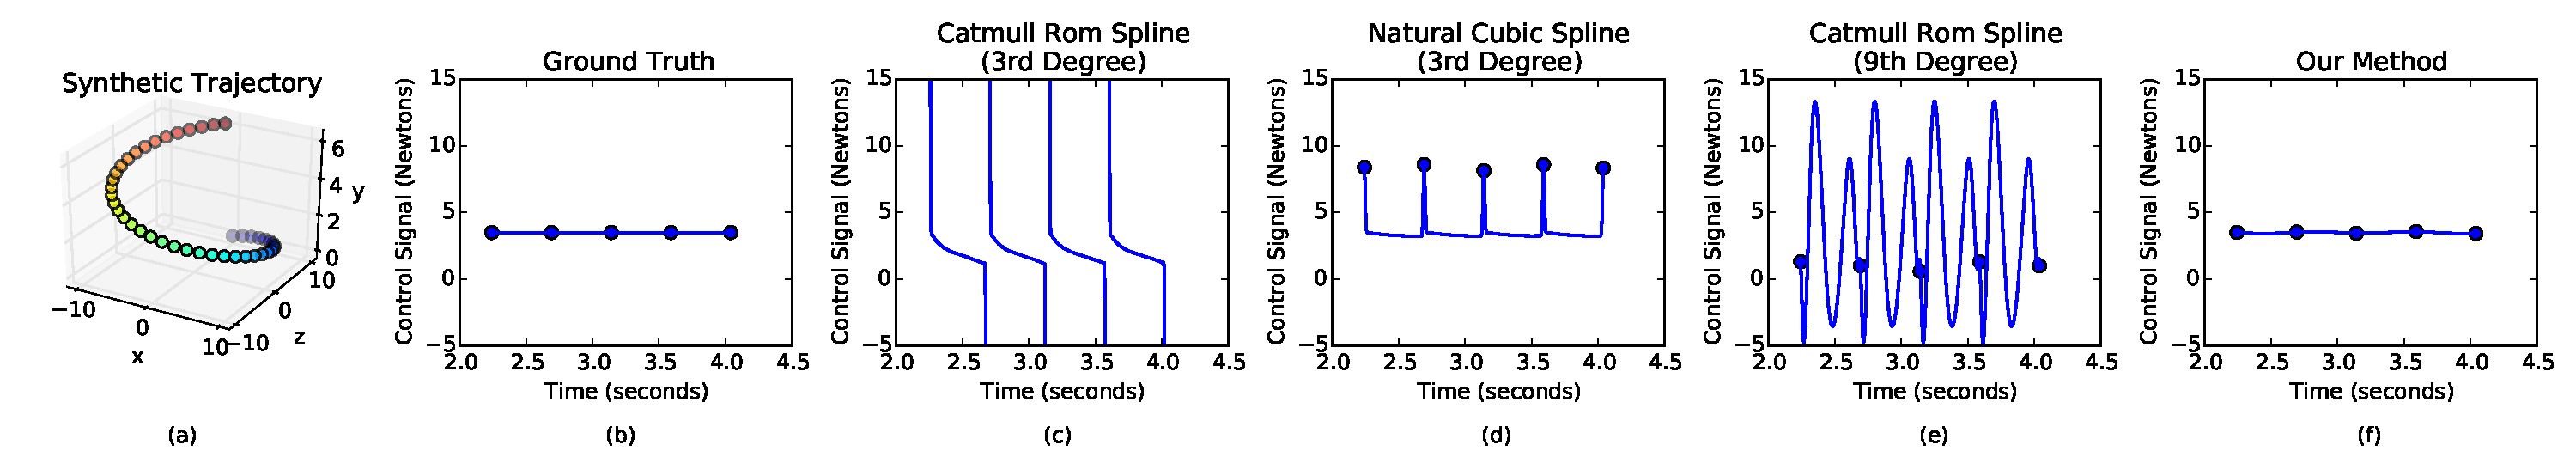
\includegraphics[width=6.0in]{images/2015_siggraph_asia_supplementary/method_comparison}
\caption{
Comparison of the quadrotor control signals resulting from different keyframe interpolation methods.
We construct a simple synthetic traejectory (a). We use the control signals required for a  quadrotor to follow the synthetic trajectory as ground truth (b).
We sample the synthetic trajectory with 15 evenly spaced keyframes, and we construct an interpolated trajectory from these keyframes using different interpolation methods.
We plot the control signals produced by each interpolation method. We require that the control signals be continuous, and we prefer control signals that are as close as possible to the ground truth. We show the middle of these control signal plots to highlight their periodic behavior without boundary artifacts.
For each interpolation method, we show the control signal for the front right propeller, and we indicate the control signal value at each keyframe with a blue dot.
\nth{3} degree Catmull Rom Splines are $C^1$ continuous, and therefore produce discontinuous control signals (c).
Natural Cubic Splines are $C^2$ continuous, and therefore also produce discontinuous control signals (d).
\nth{9} degree Catmull Rom Splines are $C^4$ continuous, so they produce continuous control signals, but with large periodic excursions (e).
Our method is $C^4$ continuous and produces control signals with minimal excursions (f). 
}
\label{fig:ch2:method_comparison}
\end{figure*}

\begin{figure*}[t!]
\centering
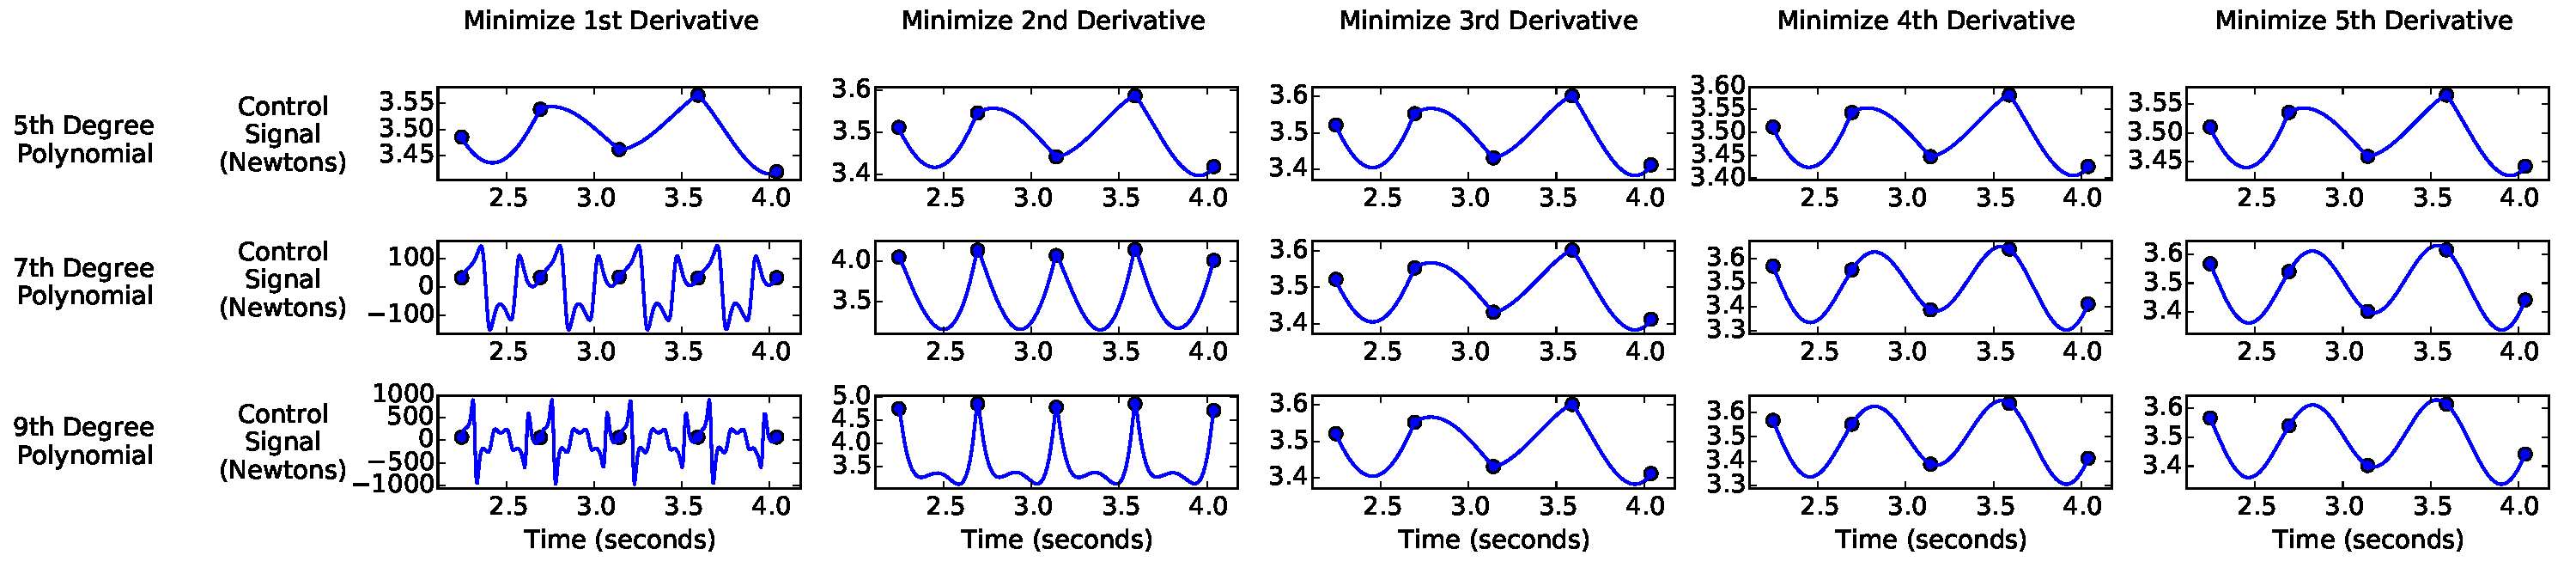
\includegraphics[width=6.0in]{images/2015_siggraph_asia_supplementary/parameter_comparison}
\caption{
Comparison of the quadrotor control signals resulting from different variations of our method when interpolating the synthetic trajectory described in Figure \ref{fig:ch2:method_comparison}.
We show the middle of these control signal plots to highlight their periodic behavior without boundary artifacts.
For each variation of our method, we show the control signal for the front right propeller, and we indicate the control signal value at each keyframe with a blue dot. Note that the vertical scaling varies in each subplot, and is different from the vertical scaling in Figure \ref{fig:ch2:method_comparison}.
Minimizing the \nth{4} derivative of \nth{7} degree polynomials (also shown, with different vertical scaling, in Figure \ref{fig:ch2:method_comparison}f) is the simplest variation of our method that produces smooth and reasonably bounded control signals.
Note that  $C^4$ continuous position trajectories are only guaranteed to produce $C^0$ continuous control signals for quadrotors, which is why some of the control signals in this figure are jagged.
}
\label{fig:ch2:parameter_comparison}
\end{figure*}

\subsection{Empirical Justification for Minimizing the \nth{4} Derivative of \nth{7} Degree Polynomials}
\label{sec:ch2:derivative_experiment}

In this subsection, we evaluate alternative polynomial representations for quadrotor camera paths.
We find that minimizing the \nth{4} derivative of \nth{7} degree piecewise polynomials produces the smoothest and most reasonably bounded control signals for quadrotors (see Figures \ref{fig:ch2:method_comparison} and \ref{fig:ch2:parameter_comparison} in this document).

When evaluating alternative polynomial representations, we chose to limit our experiments to odd degree (i.e., even order) polynomials, since these tend to produce smoother curves than even degree (i.e., odd order) polynomials \cite{goshtasby:1990}.


\subsection{Proof that B is Always Full Column Rank}
\label{sec:ch2:rank}

To prove that the matrix $\mathbf{B}$ is full column rank, consider the following matrix,
%
\begin{equation}
\mathbf{M} = 
\begin{bmatrix}
\mathbf{R}_{\mathcal{W},\mathcal{Q}} \mathbf{M}_{\mathbf{f}} \\
\mathbf{M}_{\mathbf{\tau}}                                   \\
\end{bmatrix}
\end{equation}
%
It will suffice to show that $\mathrm{rank}(\mathbf{M})=4$.
We assume without loss of generality that $0 < \alpha, \beta < \frac{\pi}{2}$ and that $d,\gamma > 0$.
We can clearly see that $\mathrm{rank}(\mathbf{M}_{\mathbf{\tau}})=3$.

Suppose for the sake of contradiction that $\mathrm{rank}(\mathbf{M})=3$.
Then we must be able to represent any row of $\mathbf{R}_{\mathcal{W},\mathcal{Q}} \mathbf{M}_{\mathbf{f}}$ as a linear combination of the rows of $\mathbf{M}_{\mathbf{\tau}}$.
Let the row $\mathbf{r} =[r ~ r ~ r ~ r]$ be one such row of $\mathbf{R}_{\mathcal{W},\mathcal{Q}} \mathbf{M}_{\mathbf{f}}$.
Representing $\mathbf{r}$ as a linear combination of the rows in $\mathbf{M}_{\mathbf{\tau}}$, we get the following system of equations,
%
\begin{equation}
\begin{aligned}
r & = ~   i ds_{\alpha} & + & ~ j \gamma & - & ~ k dc_{\alpha} \\
r & = ~   i ds_{\beta}  & - & ~ j \gamma & + & ~ k dc_{\beta}  \\
r & = ~ - i ds_{\beta}  & + & ~ j \gamma & + & ~ k dc_{\beta}  \\
r & = ~ - i ds_{\alpha} & - & ~ j \gamma & - & ~ k dc_{\alpha}
\end{aligned}
\end{equation}
%
for some $i,j,k$.
Equating the first and last of these equations above, we get $i ds_{\alpha} = - j \gamma $.
Equating the middle two of these equations above, we get $i ds_{\beta} =  j \gamma $.
Substituting these two new expressions into the first two equations above, we get $c_{\alpha} = - c_{\beta}$.
However, this is only possible if $\alpha$ or $\beta$ is outside the range $(0,\frac{\pi}{2})$.
Since we had previously assumed that $\alpha$ and $\beta$ are both inside the range $(0,\frac{\pi}{2})$, we have arrived at a contradiction.
This completes our proof.

% \section*{Acknowledgements}

% We thank Tao Du for catching and correcting an error in equation (9) in this document.

% \bibliographystyle{acmsiggraph}
% \bibliography{00_main}

% \end{document}


